\chapter {Methodology}

\section{Model Development}
\begin{enumerate}
    \item Conduct a comprehensive analysis of existing models for PoW and PoS blockchains. Select a state-of-the-art model to improve upon, ensuring it employs a bottom-up approach. This enables the possibility of incorporating new factors into it \cite{CambridgeCBECI}. Provide a comprehensive explanation of each of its components.

    \item Acquire a deep understanding of the interplay between microscopic factors and their macroscopic effects in PoS Ethereum \cite{MarionAnModelling}. With this knowledge, identify 3-4 shortcomings and limitations of the base model chosen.

    \item Considering the limited 'post-merge' data available, choose 2 of these factors to incorporate into the base model. Analyse data and literature relating these factors to electricity consumption in various contexts. Adhering to the principles of \textit{Rule-Based Mathematical Modelling}, outlined in \sref{MathematicalModellingLitRev}, develop equations related to PoS Ethereum either by adapting existing equations to the given context or through modelling the behaviours observed in the data \cite{CryptoCarbonRatingsInstitute2022TheNetwork}.

    \item Incorporate these equations into the base model. Where possible, estimate the network shares of users employing different hardware, client, and node configurations, and assign weights to different parts of the final equation \cite{CCRI:Institute}.

    \item Determine the contemporary metrics (e.g., gas fees, transaction count, etc.) required to implement the proposed model and other competing models. Apply all models using the same metrics to produce comparable values (like energy consumption per transaction) to facilitate the evaluation of the model's results \cite{CryptoCarbonRatingsInstitute2022TheNetwork}.

\end{enumerate}

\section {Evaluation Metrics}

\subsection{Quantitative}
\label{MethoologyErrorQuant}
Simulating the microscopic characteristics of PoS Ethereum that are leveraged in this study is a near-impossible task. Thus a validation metric must be chosen as a quantitative means of validating this study's results. The aim of a validation metric is to be able to assess the predictive capability of a mathematical model \cite{Kat2012ValidationError}. Most relative-error measures compare true observed values to predicted results. However, since all existing models estimate the energy consumption of Ethereum, there is no true value. Thus, selecting a suitable error measure is difficult. Most competing studies have not performed statistical significance tests or applied quantitative error measures because of insufficient data.

The relative-error measure chosen is the magnitude error, which compares the relative orders of magnitude between two functions. \eref{eqn:ErrorMeasureEqn} can be used to calculate this. Results from an experimental model with scientific data will be treated as the true values  $\boldsymbol{\mathrm{m}}$, while estimates from this study's 'Model-A' will replace prediction values $\boldsymbol{\mathrm{p}}$ \cite{RussellErrorMeasure}. The suggested upper bound for an acceptable result is $\boldsymbol{\epsilon_\mathrm{rme} \leq 0.2}$.

\begin{align}
\label{eqn:ErrorMeasureEqn}
    &\boldsymbol{\epsilon_\mathrm{rme} = \mathrm{sign(rme)} * \log_{10} (1 + |\mathrm{rme}|)}
    &\boldsymbol{ \mathrm{rme} = \mathrm{\frac{\mathrm{\sum\limits_{i=1}^{N} p_{i}^{2}} - \mathrm{\sum\limits_{i=1}^{N} m_{i}^{2}}}{\sqrt{\mathrm{\sum\limits_{i=1}^{N} p_{i}^{2}} * \mathrm{\sum\limits_{i=1}^{N} m_{i}^{2}}}}}}
\end{align}

% --------------------------------------------------------------------
\subsection{Qualitative}
\label{QualModelEvalMEthodology}
For verification of the model proposed, qualitative techniques that can be used include \cite{Al-Aomar2015ModelTechniques}:

\textbf{1. Thorough Examination of Model Inputs - } During model development, the input values for each part of the model must be obtained only from scientific sources. Where infeasible, anecdotal data from multiple sources must be averaged and used as a substitute. A 'valid' input is defined as being:
\begin{enumerate}
    \item Correct
    \item Relevant to the real-world system being modelled
    \item Being used in the model similar to the way they would be used by the real-world system
\end{enumerate}  

\textbf{2. Detailed Documentation of Model Logic - }
Every decision made during the model's development must be clearly documented and well-justified using either observed data or domain-specific knowledge. All assumptions will be highlighted using bold formatting.


\textbf{3. Thorough Examination of Model Outputs - }
The model's results must lie in a 'reasonable' range when compared to competing model's results \cite{Al-Aomar2015ModelTechniques}. Any discrepancies between Model-A and other similar models must be clearly explained in the discussion section.   

\section {Data Gathering}

The primary scientific source of data in this field is the experiment conducted in the CCRI study \cite{CryptoCarbonRatingsInstitute2022TheNetwork}, often referenced by most other studies in this emerging area of research \cite{IbanezTheExpansion}. In addition to this data, a variety of sources, including blockchain crawlers for obtaining metrics such as transaction counts, and non-empirical sources like Reddit and Discord communities (where reputed users share their electricity measurements), are collected and averaged in Appendix A.

The CCRI \cite{Ccri-apiOverview} and Etherscan \cite{EtherscanProvider} APIs will be used to pursue a data-driven approach to modelling. Most indices that are publicly accessible on the CCRI website display annualised values for daily estimates. These values will be divided by 365 to acquire accurate daily figures.

% \section {Modelling The Energy Consumption Using Domain Knowledge}

% *Define everything in your modelling world, what your definition of everything is

% We care about the power coming from the grid. The AC 'At-Wall'. We gather estimations for the recommended configuration of hardware for Ethereum nodes running validator clients. 

% Also decide on which way of data gathering is better. Prepare a table of online users claiming their power consumption. Also, estimate the power consumption of the recommended configuration of hardware through manufacturer websites. This is then compared to the data from the \cite{CryptoCarbonRatingsInstitute2022TheNetwork} report actually running a single validator node to check if this bottom-up hardware estimation approach is valid. 

% Knowing the fact that increasing the number of validator clients on a single machine increases the power consumption logarithmically, we apply this assumption to the CCRI equation. We also need to account for power inefficiency of the computer by adding a factor to this equation. The report does not mention the power supply or mainboard used.

% Also need to add the syncing energy into the equation as it is not a short process. Need to model this, depending on the data and add it to the equation. (possibly for every combination of CL and EL client)
% ------------------------------------------------------------------

\section {Project Management}

Agile project management practices were employed during the course of this project. 

\subsection{Task Management}

Given the frequent topic changes throughout the course of this project, the adoption of agile practices was critical to its success. A task management tool called Todoist was utilised for micro-task management. Its visual task board enabled task categorisation by importance level, date, and macro-tasks, as demonstrated in Appendix E. The Gantt chart was updated each time a self-set milestone dated into the Todist board was completed.

Macro-level task management was accomplished through implementing a Gantt chart. Its tasks were updated regularly due to newfound knowledge of the research area and any technical progress made. The latest Gantt chart is shown in \fref{Figure:ganttUpdated}, with the original version in Appendix G. 

\subsection{Time Management}

The Gantt chart also facilitated macro-level time allocation to major tasks, split across both academic semesters. Realistic allocations were made and updated monthly, accounting for other coursework and unexpected delays. 

Furthermore, brief summaries of all relevant literature were recorded in a Word document found in Appendix F. This approach allowed for the efficient organisation of ideas and prevented rereading papers, saving time. 


\begin{figure}[!htb]
    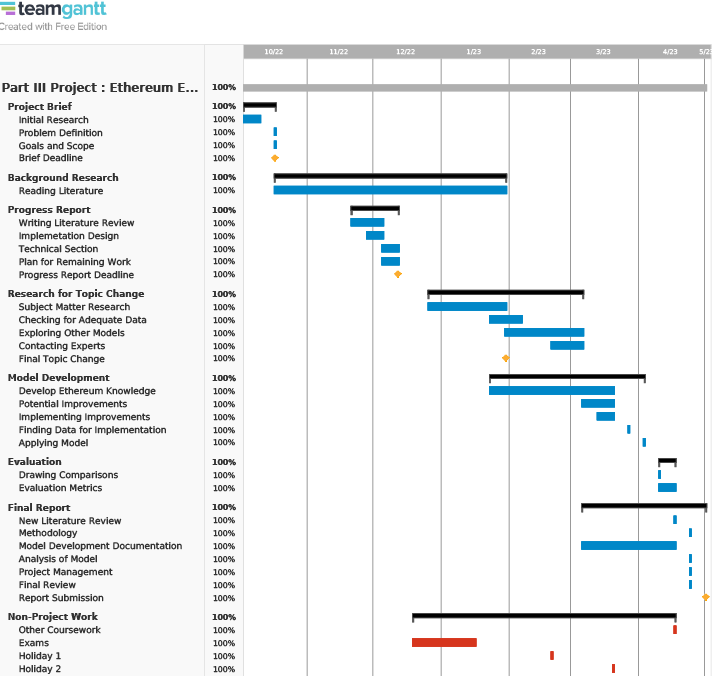
\includegraphics[width=14cm,center]{Figures/ganttUpdated.png}
    \caption{Latest version of the Gantt Chart. Older Gantt Chart found in Appendix G.}
    \label{Figure:ganttUpdated}
\end{figure}



\subsection{Risk Management}

Forseen risks associated with taking on such a novel project have been compiled into \tref{Figure:RiskTable}, ordered by descending risk score. This is calculated as the quotient of $\mathrm{Probability * Impact}$.

\begin{table}[!htb]
    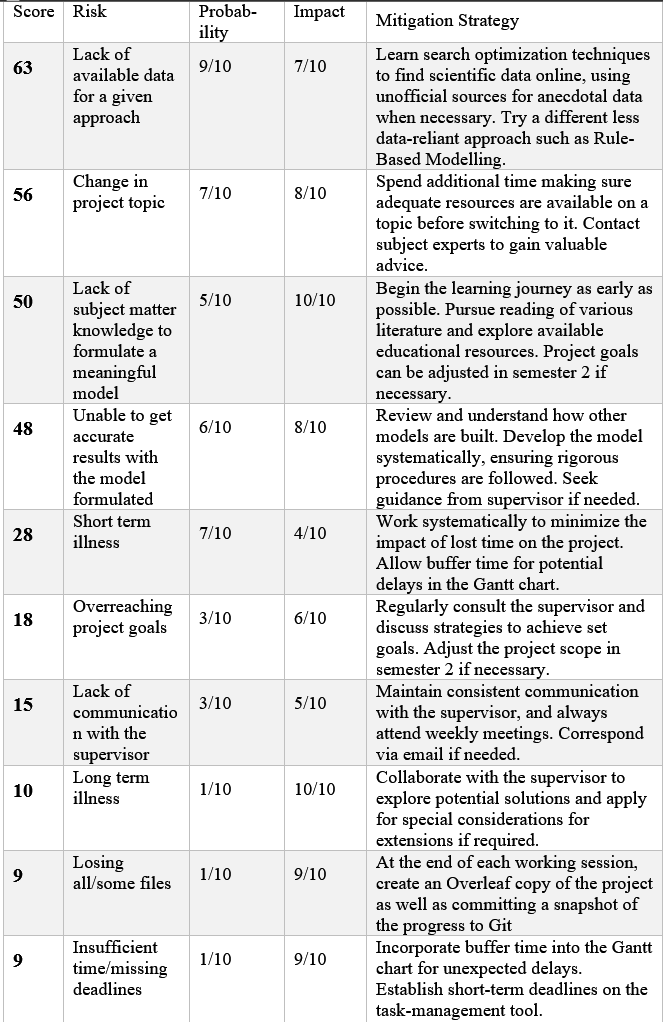
\includegraphics[width=13cm,center]{Figures/RiskTable2.png}
    \caption{Risk Analysis table (taken from the previously submitted progress report).}
    \label{Figure:RiskTable}
\end{table}